\documentclass{article}

\newcommand{\keywords}[1]{\par\noindent\textbf{Keywords:} #1}
% Language setting
% Replace `english' with e.g. `spanish' to change the document language
\usepackage[english]{babel}

% Set page size and margins
% Replace `letterpaper' with `a4paper' for UK/EU standard size
\usepackage[letterpaper,top=2cm,bottom=2cm,left=3cm,right=3cm,marginparwidth=1.75cm]{geometry}
\usepackage{tikz}
\usepackage{pgfplots}
\usetikzlibrary{arrows.meta}
% Useful packages
\usepackage{amsmath}
\usepackage{graphicx}
\usepackage{booktabs}
\usepackage[linesnumbered,ruled,vlined]{algorithm2e}
\usepackage[colorlinks=true, allcolors=blue]{hyperref}
\SetKw{KwDownTo}{down to}

\title{simple cache-sentive skip list}

\author[1]{Yuchang Ke}
\author[2]{Bill Lv}
\author[3]{Weijie Zhang}

\email[1]{aceking.ke@gmail.com}
\email[2]{ideaalloc@gmail.com}
\email[3]{zhangweijie@gmail.com}

\affil[1]{%
  \institution{} 
  \streetaddress{}
  \city{Wuhan}
  \state{China}
  \postcode{430000}
}
\affil[2]{%
  \institution{} 
  \streetaddress{}
  \city{Wuhan}
  \state{China}
  \postcode{430000}
}
\affil[3]{%
  \institution{Hubei Changjiang Yunxin Media Group Co., Ltd} 
  \streetaddress{No. 788, Gaoxin Ave., Hubei Broadcasting&TV Media Tower}
  \city{Wuhan}
  \state{China}
  \postcode{430000}
}

\begin{document}
\maketitle

\begin{abstract}
      We present a cache-sensitive skiplist that is very simple and easy to implement. It only requires a few small modifications to the original skiplist to adapt it to modern CPU architectures, resulting in a performance improvement of 1.2~1.6 times, in some system it can reach 2X or 3X.
      Unlike other optimizations, it does not require specialized instructions such as SIMD or multi-threaded programming. Instead, it takes advantage of modern compiler optimizations, making it more universal. This design can be used not only in in-memory databases or key-value stores, but also in embedded systems.

\keywords{skiplist; cache-sensitive; index structure}
\end{abstract}



\section{Introduction}

In the field of computer science, ordered data structures are a fundamental tool for organizing and managing data. Efficient execution of search, delete, and insert operations is crucial for a wide range of applications, as it directly impacts overall system performance.
To achieve high performance in ordered data structures, many methods have been developed, such as AVL trees and Red-Black trees. However, these structures are relatively complex due to the need for rebalancing. This changed when William Pugh introduced the skip list in 1990\cite{ref1}. It introduced a randomized data structure that simplified implementation compared to traditional balanced trees.

Thanks to its simplicity, the skip list has been adopted by various systems, including databases such as LevelDB\cite{ref2}, Redis\cite{ref7}, and RocksDB\cite{ref3}, Hbase\cite{ref4} in-memory caches, and the inverted index in Lucene.

Skip list can be divided into multiple levels, one data level and multiple index levels. Data level is the lowest level(level 0), which stores all the data nodes. And the index levels provide short paths to access the data node at the data level, and all the levels are linked lists. Because of this, these data nodes and index nodes are non-contiguous in memory address. This causes the performance to be degraded by cache misses.
Although ESL, CSSL has developed cache sensitive skip lists to fit modern CPU architecture, these algorithms are still complex, and CSSL uses SIMD instructions which are special in Intel. We strongly believe that the value of a skiplist lies in its simplicity.  Excessively complex cache-sensitive designs reduce the appeal of skip list variations.

With the emergence of new technologies and computing architectures, particularly multi-core CPUs and vectorization, novel variants of skip lists have been developed. Such as Cache-Sensitive Skiplist (CSSL)\cite{ref5}, which merges nodes at the index level into a single array, which are named fast lanes, and all nodes in the fast lane are sorted. This design is more cache-friendly. It also uses SIMD instructions, ESL( A High-Performance Skiplist with Express Lane\cite{ref6})  also merges the nodes in index levels into a single array, and they use version-based lock protocol and lock-free operation log to implement concurrency. 


\section{Design overview}

In this paper, we present a simple and easy-to-implement cache-sensitive skip list. At the data level, it introduces a vector, and the nodes at this level now store arrays instead of single values. Leveraging CPU cache benefits for small arrays to enhance skip list performance. For example, consider a skip list with a vector at the data level; let's suppose the vector's maximum size is 2, as shown in Figure 1. 

There are 3 key points: 1) At the data level, we use a sorted array with a fixed maximum length. Since the keys are integers, we choose a maximum length of 128 or less. 2) For all index levels, we use only the first element of the array as a pivot for comparison. 3) The last element of the array is considered solely during insertion operations, and only under particular conditions.

\begin{figure}[h]
\centering
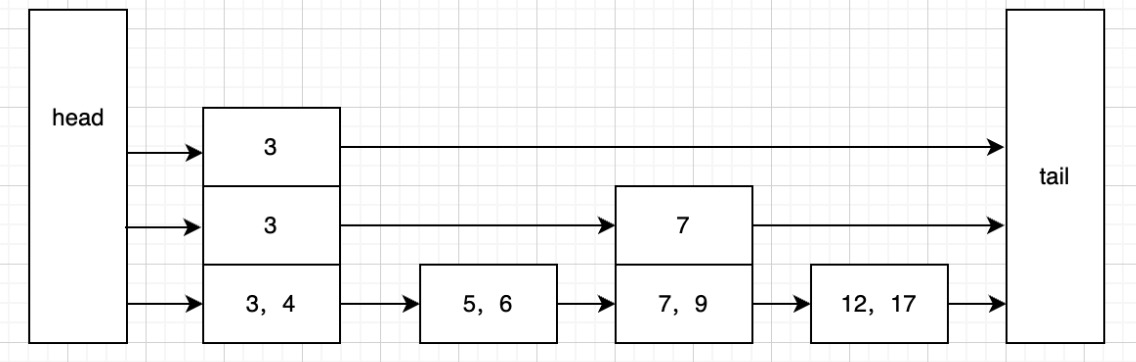
\includegraphics[width=0.5\linewidth]{skiplist.png}
\caption{A simple cache-sensitive skip list}
\label{fig:fig1}
\end{figure}
Our key contributions include: 1. Introducing a vector, which maintains the algorithm's complexity while improving CPU cache hit rate due to its contiguous storage. 2. Reducing the skiplist's level count and pointer overhead by incorporating a vector. 3. Presenting vector-based insertion, search, and deletion algorithms for data nodes, offering a novel perspective for database index design.

\section{Algorithm}
This section gives the algorithm for search, insertion, and deletion. The insertion operation inserts new specified data into the data structure, and the search operation finds data and returns it. The deletion operation deletes data. 

In SCSSL, at the data level, data is stored in a single array with a fixed maximum size. As the same as the standard skip list, the level of the node is chosen randomly when the node is created. And a level i node has the same number of forward pointers (also i), the maximum of levels is a constant MaxLevel. It also has a header that leads the search of the data structure, and the last nodes of all levels’ forward pointers point to NIL.


\begin{figure}[ht]
      \centering
\tikzset{every picture/.style={line width=0.75pt}} %set default line width to 0.75pt        

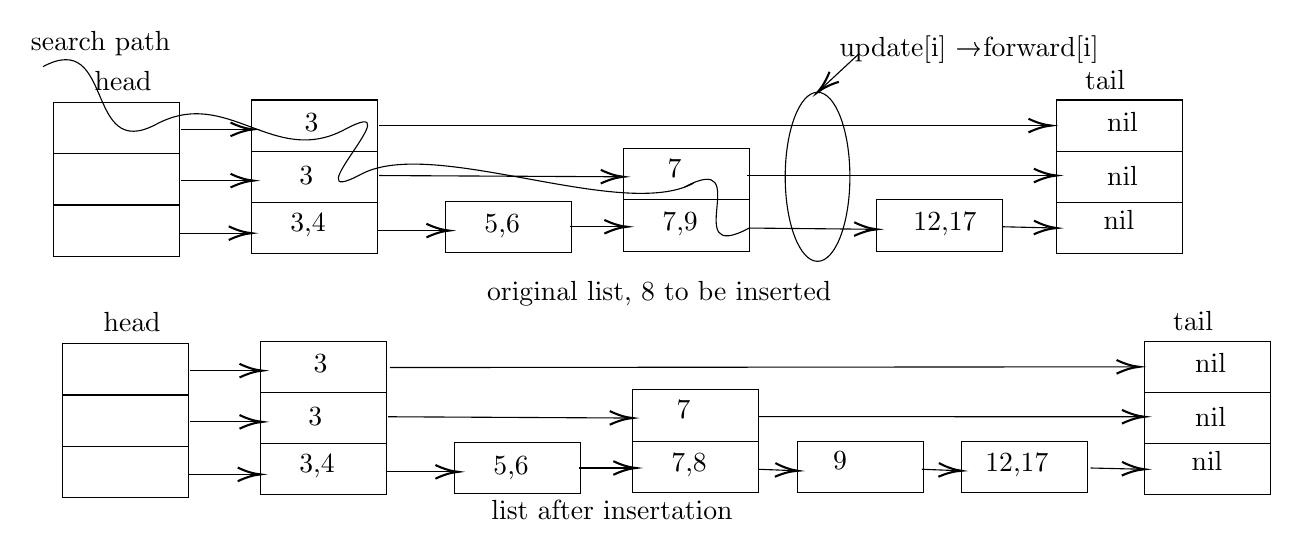
\begin{tikzpicture}[x=0.75pt,y=0.75pt,yscale=-1,xscale=1]
%uncomment if require: \path (0,302); %set diagram left start at 0, and has height of 302

%Shape: Rectangle [id:dp802121456728152] 
\draw   (57.79,105.64) -- (118.41,105.64) -- (118.41,130.32) -- (57.79,130.32) -- cycle ;
%Shape: Rectangle [id:dp9825705095547612] 
\draw   (332.28,103.17) -- (392.89,103.17) -- (392.89,127.86) -- (332.28,127.86) -- cycle ;
%Shape: Rectangle [id:dp248949237262718] 
\draw   (246.56,103.79) -- (307.17,103.79) -- (307.17,128.47) -- (246.56,128.47) -- cycle ;
%Shape: Rectangle [id:dp1628354408576529] 
\draw   (153.04,104.41) -- (213.65,104.41) -- (213.65,129.09) -- (153.04,129.09) -- cycle ;
%Shape: Rectangle [id:dp000018829587681290505] 
\draw   (57.79,56.27) -- (118.41,56.27) -- (118.41,80.96) -- (57.79,80.96) -- cycle ;
%Shape: Rectangle [id:dp247562625981687] 
\draw   (57.79,80.96) -- (118.41,80.96) -- (118.41,105.64) -- (57.79,105.64) -- cycle ;
%Shape: Rectangle [id:dp2644216550992282] 
\draw   (540.96,104.41) -- (601.57,104.41) -- (601.57,129.09) -- (540.96,129.09) -- cycle ;
%Shape: Rectangle [id:dp8347359895416517] 
\draw   (540.96,55.04) -- (601.57,55.04) -- (601.57,79.72) -- (540.96,79.72) -- cycle ;
%Shape: Rectangle [id:dp6823901202027933] 
\draw   (540.96,79.72) -- (601.57,79.72) -- (601.57,104.41) -- (540.96,104.41) -- cycle ;
%Shape: Rectangle [id:dp379773497534003] 
\draw   (153.04,79.72) -- (213.65,79.72) -- (213.65,104.41) -- (153.04,104.41) -- cycle ;
%Shape: Rectangle [id:dp8262463980956687] 
\draw   (153.04,55.04) -- (213.65,55.04) -- (213.65,79.72) -- (153.04,79.72) -- cycle ;
%Shape: Rectangle [id:dp618442800182132] 
\draw   (454.37,103.17) -- (514.98,103.17) -- (514.98,127.86) -- (454.37,127.86) -- cycle ;
%Straight Lines [id:da18234761053431092] 
\draw    (118.41,119.22) -- (151.04,119.22) ;
\draw [shift={(153.04,119.22)}, rotate = 180] [color={rgb, 255:red, 0; green, 0; blue, 0 }  ][line width=0.75]    (10.93,-3.29) .. controls (6.95,-1.4) and (3.31,-0.3) .. (0,0) .. controls (3.31,0.3) and (6.95,1.4) .. (10.93,3.29)   ;
%Straight Lines [id:da17691354593928432] 
\draw    (213.65,117.98) -- (246.29,117.98) ;
\draw [shift={(248.29,117.98)}, rotate = 180] [color={rgb, 255:red, 0; green, 0; blue, 0 }  ][line width=0.75]    (10.93,-3.29) .. controls (6.95,-1.4) and (3.31,-0.3) .. (0,0) .. controls (3.31,0.3) and (6.95,1.4) .. (10.93,3.29)   ;
%Straight Lines [id:da06545360607750506] 
\draw    (306.3,116.13) -- (332.01,116.13) ;
\draw [shift={(334.01,116.13)}, rotate = 180] [color={rgb, 255:red, 0; green, 0; blue, 0 }  ][line width=0.75]    (10.93,-3.29) .. controls (6.95,-1.4) and (3.31,-0.3) .. (0,0) .. controls (3.31,0.3) and (6.95,1.4) .. (10.93,3.29)   ;
%Straight Lines [id:da8917793267177494] 
\draw    (392.89,116.75) -- (452.37,117.34) ;
\draw [shift={(454.37,117.36)}, rotate = 180.58] [color={rgb, 255:red, 0; green, 0; blue, 0 }  ][line width=0.75]    (10.93,-3.29) .. controls (6.95,-1.4) and (3.31,-0.3) .. (0,0) .. controls (3.31,0.3) and (6.95,1.4) .. (10.93,3.29)   ;
%Straight Lines [id:da6270688079351094] 
\draw    (514.98,116.13) -- (538.96,116.7) ;
\draw [shift={(540.96,116.75)}, rotate = 181.36] [color={rgb, 255:red, 0; green, 0; blue, 0 }  ][line width=0.75]    (10.93,-3.29) .. controls (6.95,-1.4) and (3.31,-0.3) .. (0,0) .. controls (3.31,0.3) and (6.95,1.4) .. (10.93,3.29)   ;
%Straight Lines [id:da16483082426708995] 
\draw    (119.27,93.91) -- (151.91,93.91) ;
\draw [shift={(153.91,93.91)}, rotate = 180] [color={rgb, 255:red, 0; green, 0; blue, 0 }  ][line width=0.75]    (10.93,-3.29) .. controls (6.95,-1.4) and (3.31,-0.3) .. (0,0) .. controls (3.31,0.3) and (6.95,1.4) .. (10.93,3.29)   ;
%Shape: Rectangle [id:dp8280971824764716] 
\draw   (332.28,78.49) -- (392.89,78.49) -- (392.89,103.17) -- (332.28,103.17) -- cycle ;
%Straight Lines [id:da6251582090553987] 
\draw    (119.27,69.23) -- (151.91,69.23) ;
\draw [shift={(153.91,69.23)}, rotate = 180] [color={rgb, 255:red, 0; green, 0; blue, 0 }  ][line width=0.75]    (10.93,-3.29) .. controls (6.95,-1.4) and (3.31,-0.3) .. (0,0) .. controls (3.31,0.3) and (6.95,1.4) .. (10.93,3.29)   ;
%Straight Lines [id:da906622887317923] 
\draw    (214.52,67.38) -- (536.36,67.38) ;
\draw [shift={(538.36,67.38)}, rotate = 180] [color={rgb, 255:red, 0; green, 0; blue, 0 }  ][line width=0.75]    (10.93,-3.29) .. controls (6.95,-1.4) and (3.31,-0.3) .. (0,0) .. controls (3.31,0.3) and (6.95,1.4) .. (10.93,3.29)   ;
%Straight Lines [id:da1247883464855224] 
\draw    (214.52,91.45) -- (330.28,92.05) ;
\draw [shift={(332.28,92.06)}, rotate = 180.3] [color={rgb, 255:red, 0; green, 0; blue, 0 }  ][line width=0.75]    (10.93,-3.29) .. controls (6.95,-1.4) and (3.31,-0.3) .. (0,0) .. controls (3.31,0.3) and (6.95,1.4) .. (10.93,3.29)   ;
%Straight Lines [id:da5312111106538793] 
\draw    (392.03,91.45) -- (538.96,91.45) ;
\draw [shift={(540.96,91.45)}, rotate = 180] [color={rgb, 255:red, 0; green, 0; blue, 0 }  ][line width=0.75]    (10.93,-3.29) .. controls (6.95,-1.4) and (3.31,-0.3) .. (0,0) .. controls (3.31,0.3) and (6.95,1.4) .. (10.93,3.29)   ;
%Curve Lines [id:da7690346774156931] 
\draw    (107.15,66.76) .. controls (141.78,48.25) and (163.43,87.74) .. (198.07,69.23) ;
%Curve Lines [id:da09969258339888487] 
\draw    (198.07,69.23) .. controls (232.7,50.72) and (171.22,109.34) .. (205.86,90.83) ;
%Curve Lines [id:da17301735066569246] 
\draw    (205.86,90.83) .. controls (240.5,72.32) and (331.41,113.66) .. (366.05,95.15) ;
%Curve Lines [id:da04935924618461396] 
\draw    (361.72,97) .. controls (396.36,78.49) and (358.26,135.26) .. (392.89,116.75) ;
%Curve Lines [id:da43861108104506963] 
\draw    (52.6,38.99) .. controls (87.23,20.48) and (72.51,85.27) .. (107.15,66.76) ;
%Shape: Ellipse [id:dp551323556779669] 
\draw   (410.21,92.06) .. controls (410.21,69.57) and (417.19,51.33) .. (425.8,51.33) .. controls (434.4,51.33) and (441.38,69.57) .. (441.38,92.06) .. controls (441.38,114.56) and (434.4,132.79) .. (425.8,132.79) .. controls (417.19,132.79) and (410.21,114.56) .. (410.21,92.06) -- cycle ;
%Straight Lines [id:da9115207752269137] 
\draw    (445.71,32.82) -- (427.26,49.97) ;
\draw [shift={(425.8,51.33)}, rotate = 317.09] [color={rgb, 255:red, 0; green, 0; blue, 0 }  ][line width=0.75]    (10.93,-3.29) .. controls (6.95,-1.4) and (3.31,-0.3) .. (0,0) .. controls (3.31,0.3) and (6.95,1.4) .. (10.93,3.29)   ;
%Shape: Rectangle [id:dp44944938443713855] 
\draw   (62.12,221.87) -- (122.73,221.87) -- (122.73,246.55) -- (62.12,246.55) -- cycle ;
%Shape: Rectangle [id:dp8751335667917544] 
\draw   (336.61,219.4) -- (397.22,219.4) -- (397.22,244.08) -- (336.61,244.08) -- cycle ;
%Shape: Rectangle [id:dp2257346710215089] 
\draw   (250.89,220.01) -- (311.5,220.01) -- (311.5,244.7) -- (250.89,244.7) -- cycle ;
%Shape: Rectangle [id:dp8771184949651254] 
\draw   (157.37,220.63) -- (217.98,220.63) -- (217.98,245.32) -- (157.37,245.32) -- cycle ;
%Shape: Rectangle [id:dp5789469841235695] 
\draw   (62.12,172.5) -- (122.73,172.5) -- (122.73,197.18) -- (62.12,197.18) -- cycle ;
%Shape: Rectangle [id:dp5624687649592586] 
\draw   (62.12,197.18) -- (122.73,197.18) -- (122.73,221.87) -- (62.12,221.87) -- cycle ;
%Shape: Rectangle [id:dp13120546674792055] 
\draw   (583.39,220.63) -- (644,220.63) -- (644,245.32) -- (583.39,245.32) -- cycle ;
%Shape: Rectangle [id:dp18910975661576046] 
\draw   (583.39,171.26) -- (644,171.26) -- (644,195.95) -- (583.39,195.95) -- cycle ;
%Shape: Rectangle [id:dp968839873549274] 
\draw   (583.39,195.95) -- (644,195.95) -- (644,220.63) -- (583.39,220.63) -- cycle ;
%Shape: Rectangle [id:dp5100738159249718] 
\draw   (157.37,195.95) -- (217.98,195.95) -- (217.98,220.63) -- (157.37,220.63) -- cycle ;
%Shape: Rectangle [id:dp5130816669129519] 
\draw   (157.37,171.26) -- (217.98,171.26) -- (217.98,195.95) -- (157.37,195.95) -- cycle ;
%Shape: Rectangle [id:dp10069788621732956] 
\draw   (495.07,219.4) -- (555.68,219.4) -- (555.68,244.08) -- (495.07,244.08) -- cycle ;
%Straight Lines [id:da7506949131852723] 
\draw    (122.73,235.44) -- (155.37,235.44) ;
\draw [shift={(157.37,235.44)}, rotate = 180] [color={rgb, 255:red, 0; green, 0; blue, 0 }  ][line width=0.75]    (10.93,-3.29) .. controls (6.95,-1.4) and (3.31,-0.3) .. (0,0) .. controls (3.31,0.3) and (6.95,1.4) .. (10.93,3.29)   ;
%Straight Lines [id:da5055411274108006] 
\draw    (217.98,234.21) -- (250.62,234.21) ;
\draw [shift={(252.62,234.21)}, rotate = 180] [color={rgb, 255:red, 0; green, 0; blue, 0 }  ][line width=0.75]    (10.93,-3.29) .. controls (6.95,-1.4) and (3.31,-0.3) .. (0,0) .. controls (3.31,0.3) and (6.95,1.4) .. (10.93,3.29)   ;
%Straight Lines [id:da7559298876477776] 
\draw    (310.63,232.36) -- (336.34,232.36) ;
\draw [shift={(338.34,232.36)}, rotate = 180] [color={rgb, 255:red, 0; green, 0; blue, 0 }  ][line width=0.75]    (10.93,-3.29) .. controls (6.95,-1.4) and (3.31,-0.3) .. (0,0) .. controls (3.31,0.3) and (6.95,1.4) .. (10.93,3.29)   ;
%Straight Lines [id:da08581070094109111] 
\draw    (397.22,232.97) -- (414.27,233.62) ;
\draw [shift={(416.27,233.7)}, rotate = 182.18] [color={rgb, 255:red, 0; green, 0; blue, 0 }  ][line width=0.75]    (10.93,-3.29) .. controls (6.95,-1.4) and (3.31,-0.3) .. (0,0) .. controls (3.31,0.3) and (6.95,1.4) .. (10.93,3.29)   ;
%Straight Lines [id:da5858905620692174] 
\draw    (557.41,232.36) -- (581.39,232.93) ;
\draw [shift={(583.39,232.97)}, rotate = 181.36] [color={rgb, 255:red, 0; green, 0; blue, 0 }  ][line width=0.75]    (10.93,-3.29) .. controls (6.95,-1.4) and (3.31,-0.3) .. (0,0) .. controls (3.31,0.3) and (6.95,1.4) .. (10.93,3.29)   ;
%Straight Lines [id:da32674036346427937] 
\draw    (123.6,210.14) -- (156.24,210.14) ;
\draw [shift={(158.24,210.14)}, rotate = 180] [color={rgb, 255:red, 0; green, 0; blue, 0 }  ][line width=0.75]    (10.93,-3.29) .. controls (6.95,-1.4) and (3.31,-0.3) .. (0,0) .. controls (3.31,0.3) and (6.95,1.4) .. (10.93,3.29)   ;
%Shape: Rectangle [id:dp026479095509071682] 
\draw   (336.61,194.71) -- (397.22,194.71) -- (397.22,219.4) -- (336.61,219.4) -- cycle ;
%Straight Lines [id:da5236391813651351] 
\draw    (123.6,185.46) -- (156.24,185.46) ;
\draw [shift={(158.24,185.46)}, rotate = 180] [color={rgb, 255:red, 0; green, 0; blue, 0 }  ][line width=0.75]    (10.93,-3.29) .. controls (6.95,-1.4) and (3.31,-0.3) .. (0,0) .. controls (3.31,0.3) and (6.95,1.4) .. (10.93,3.29)   ;
%Straight Lines [id:da951241427709963] 
\draw    (219.71,183.96) -- (578.79,183.61) ;
\draw [shift={(580.79,183.61)}, rotate = 179.94] [color={rgb, 255:red, 0; green, 0; blue, 0 }  ][line width=0.75]    (10.93,-3.29) .. controls (6.95,-1.4) and (3.31,-0.3) .. (0,0) .. controls (3.31,0.3) and (6.95,1.4) .. (10.93,3.29)   ;
%Straight Lines [id:da5677734486818795] 
\draw    (218.85,207.67) -- (334.61,208.28) ;
\draw [shift={(336.61,208.29)}, rotate = 180.3] [color={rgb, 255:red, 0; green, 0; blue, 0 }  ][line width=0.75]    (10.93,-3.29) .. controls (6.95,-1.4) and (3.31,-0.3) .. (0,0) .. controls (3.31,0.3) and (6.95,1.4) .. (10.93,3.29)   ;
%Straight Lines [id:da03778045413284792] 
\draw    (397.22,207.61) -- (581.39,207.67) ;
\draw [shift={(583.39,207.67)}, rotate = 180.02] [color={rgb, 255:red, 0; green, 0; blue, 0 }  ][line width=0.75]    (10.93,-3.29) .. controls (6.95,-1.4) and (3.31,-0.3) .. (0,0) .. controls (3.31,0.3) and (6.95,1.4) .. (10.93,3.29)   ;
%Shape: Rectangle [id:dp9874088035206192] 
\draw   (416.27,219.4) -- (476.88,219.4) -- (476.88,244.08) -- (416.27,244.08) -- cycle ;
%Straight Lines [id:da719219755060643] 
\draw    (476.02,232.97) -- (493.07,233.62) ;
\draw [shift={(495.07,233.7)}, rotate = 182.18] [color={rgb, 255:red, 0; green, 0; blue, 0 }  ][line width=0.75]    (10.93,-3.29) .. controls (6.95,-1.4) and (3.31,-0.3) .. (0,0) .. controls (3.31,0.3) and (6.95,1.4) .. (10.93,3.29)   ;

% Text Node
\draw (170.55,108.56) node [anchor=north west][inner sep=0.75pt]   [align=left] {3,4};
% Text Node
\draw (264.06,109.17) node [anchor=north west][inner sep=0.75pt]   [align=left] {5,6};
% Text Node
\draw (349.79,107.94) node [anchor=north west][inner sep=0.75pt]   [align=left] {7,9};
% Text Node
\draw (470.74,107.94) node [anchor=north west][inner sep=0.75pt]   [align=left] {12,17};
% Text Node
\draw (174.82,85.72) node [anchor=north west][inner sep=0.75pt]   [align=left] {3};
% Text Node
\draw (177.41,60.42) node [anchor=north west][inner sep=0.75pt]   [align=left] {3};
% Text Node
\draw (352.32,82.64) node [anchor=north west][inner sep=0.75pt]   [align=left] {7};
% Text Node
\draw (76.23,40.06) node [anchor=north west][inner sep=0.75pt]   [align=left] {head};
% Text Node
\draw (553.41,39.44) node [anchor=north west][inner sep=0.75pt]   [align=left] {tail};
% Text Node
\draw (564.06,59.8) node [anchor=north west][inner sep=0.75pt]   [align=left] {nil};
% Text Node
\draw (564.06,85.72) node [anchor=north west][inner sep=0.75pt]   [align=left] {nil};
% Text Node
\draw (562.33,106.7) node [anchor=north west][inner sep=0.75pt]   [align=left] {nil};
% Text Node
\draw (45.5,20.51) node [anchor=north west][inner sep=0.75pt]   [align=left] {search path};
% Text Node
\draw (435.12,22.78) node [anchor=north west][inner sep=0.75pt]   [align=left] {update[i] →forward[i] };
% Text Node
\draw (265.32,141.26) node [anchor=north west][inner sep=0.75pt]   [align=left] {original list, 8 to be inserted};
% Text Node
\draw (174.88,224.78) node [anchor=north west][inner sep=0.75pt]   [align=left] {3,4};
% Text Node
\draw (268.39,225.4) node [anchor=north west][inner sep=0.75pt]   [align=left] {5,6};
% Text Node
\draw (354.12,224.17) node [anchor=north west][inner sep=0.75pt]   [align=left] {7,8};
% Text Node
\draw (505.37,224.17) node [anchor=north west][inner sep=0.75pt]   [align=left] {12,17};
% Text Node
\draw (179.15,201.95) node [anchor=north west][inner sep=0.75pt]   [align=left] {3};
% Text Node
\draw (181.74,176.65) node [anchor=north west][inner sep=0.75pt]   [align=left] {3};
% Text Node
\draw (356.65,198.86) node [anchor=north west][inner sep=0.75pt]   [align=left] {7};
% Text Node
\draw (80.56,156.28) node [anchor=north west][inner sep=0.75pt]   [align=left] {head};
% Text Node
\draw (595.83,155.67) node [anchor=north west][inner sep=0.75pt]   [align=left] {tail};
% Text Node
\draw (606.49,176.03) node [anchor=north west][inner sep=0.75pt]   [align=left] {nil};
% Text Node
\draw (606.49,201.95) node [anchor=north west][inner sep=0.75pt]   [align=left] {nil};
% Text Node
\draw (604.76,222.93) node [anchor=north west][inner sep=0.75pt]   [align=left] {nil};
% Text Node
\draw (431.99,223.16) node [anchor=north west][inner sep=0.75pt]   [align=left] {9};
% Text Node
\draw (267.41,246.44) node [anchor=north west][inner sep=0.75pt]   [align=left] {list after insertation};

\end{tikzpicture}
\caption{insert 8 into simple cache-sentive skip list(max array size =2)}
\label{fig:fig2}
\end{figure}

\subsection{Initialization}
The initialization operator is elementary, just create a header with MaxLevel forwards array, and set them to Nil. To simplify the algorithm, we set the header's array with a single value, -inf.


\subsection{Search}
\begin{algorithm}[H]
    \caption{Search Key in simple cache-sentive skip list}
    \KwIn{Key $k$}
    \KwOut{Node containing key or Nil}
    \SetKwFunction{FMain}{search}
    \SetKwProg{Fn}{Function}{:}{}
    \Fn{\FMain{$k$}}{
        $current \gets header$\;
        
        \For{$i \gets level$ \KwDownTo $0$}{
            \While{$current.forward[i] \neq \text{Nil} \land current.forward[i].Key() \leq k$}{
                $current \gets current.forward[i]$\;
            }
        }
        
        \KwRet{$current.search\_in\_array(k)$}\;
    }
    \end{algorithm}

As the algorithm shows in Algorithm 1, from line 3 to line 5, it’s very similar to a standard skip list, but in line 4,current.forward[i].Key() returns the least value(at the first position) of the array in the current.forward[i]. Out of the while loop, the current’s forward Key() must be just greater than key, and if the key exists in the data structure, it must be in the current node array, so just search in the array of the current node in line 6.


\subsection{Insertion}
\begin{algorithm}[H]
    \caption{Insert Key into simple cache-sentive skip list}
    \KwIn{Key $k$}
    \KwOut{Nil}
    \SetKwFunction{FMain}{insert}
    \SetKwProg{Fn}{Function}{:}{}
    \Fn{\FMain{$k$}}{
        $update \gets \text{array of size } (max\_level + 1)$\;
        $current \gets header$\;
        
        \For{$i \gets \texttt{level}$ \KwDownTo $0$}{
            \While{$current.forward[i] \neq \text{Nil} \land current.forward[i].Key() \leq k$}{
                $current \gets current.forward[i]$\;
            }
            $update[i] \gets current$\;
        }
        
        \If{$current \neq header \land current.is\_full() \land current.array[-1] > k$}{
            $replace \gets current.array.pop()$\;
            $current.insert\_into\_array(k)$\;
            $k \gets replace$\;
        }
        
        \If{$current \neq header \land \neg current.is\_full()$}{
            $current.insert\_into\_array(k)$\;
        }
        \Else{
            $current \gets current.forward[0]$\;
            \If{$current \neq \text{Nil} \land current \neq header \land \neg current.is\_full()$}{
                $current.insert\_into\_array(k)$\;
                \KwRet{}
            }
            
            $new\_level \gets random\_level()$\;
            
            \If{$new\_level > level$}{
                \For{$i \gets level + 1 \KwDownTo new\_level$}{
                    $update[i] \gets header$\;
                }
                $level \gets new\_level$\;
            }
            
            $new\_node \gets Node([k], new\_level)$\;
            
            \For{$i \gets 0 $ \KwTo $new\_level$}{
                $new\_node.forward[i] \gets update[i].forward[i]$\;
                $update[i].forward[i] \gets new\_node$\;
            }
        }
    }
    \end{algorithm}
In Algorithm 2, from line 2 to line 7, it’s the same as a standard skip list. However, from line 8 to line 18, It should consider that level 0 nodes have a array. So there are several constraints which cannot be ignored:

\begin{itemize}


\item  If the current node is a header, a new node should be created to insert the key. We don’t want to insert data in the header; otherwise, it will be trouble for the deletion operation. So, in line 8-18, we exclude the header.
  
There are some cases for insertion:

\item CASE 1: current is not header, but current array size reach the maximum size(current.is\_full() function to check it) and key value is between the least element (first position, Key() return it) and the largest element(last position, current.array[-1]). So in this case, current node’s array is full, we make a small strick to deal with it, we pop the last position element, so the array is not full, and we insert the key in current node array(line 9,10) and it must be full again.then go on the next steps(for example, we replace 9 with 8 , and then insert 9 in another node, see Figure 2).

\item CASE 2: current is not header, current node’s array is not full, just insert the key in the array(line 12, 13). Then the insertion operation is finished.

\item CASE 3: The key is lower than current.forward’s the least value of its array(ines 4-7 has insurance for this), and the key is greater than the largest element of current node’s array, So this key should be inserted into the current’s forward node. We just insert it when the node is not full (from line 15-18), and we do not pop last element like line 9-11, for just to be simple.
\item Other CASES:  we should create a new node and insert the key in its array , and modify the forward pointers(from line 19 to 27)
\end{itemize}

\subsection{Deletion}

\begin{algorithm}[H]
        \caption{Delete key from simple cache-sentive skip list}
        \KwIn{Key $k$}
        \KwOut{True if deleted, False otherwise}
        \SetKwFunction{FMain}{delete}
        \SetKwProg{Fn}{Function}{:}{}
        \Fn{\FMain{$k$}}{
            $update \gets \text{array of size } (max\_level + 1)$\;
            $current \gets header$\;
            
            \For{$i \gets level$ \KwDownTo $0$}{
                \While{$current.forward[i] \neq \text{Nil} \land current.forward[i].array[-1] < k$}{
                    $current \gets current.forward[i]$\;
                }
                $update[i] \gets current$\;
            }
            
            $current \gets current.forward[0]$\;
            \If{$current = \text{Nil}$}{
                \KwRet{False}\;
            }
            \Else{
                $res \gets current.delete\_from\_array(k)$\;
                \If{$\neg res$}{
                    \KwRet{False}\;
                }
            }
            
            \If{$\text{len}(current.array) = 0$}{
                \For{$i \gets$ 0 $\KwTo$ $level$}{
                    \If{$update[i].forward[i] \neq current$}{
                        \textbf{break}; % Use KwBreak instead of Break
                    }
                    $update[i].forward[i] \gets current.forward[i]$\;
                }
                
                \While{$level > 0 \land header.forward[level] = \text{Nil}$}{
                    $level \gets level - 1$\;
                }
                \KwRet{True}\;
            }
        }
        \end{algorithm}
    



The deletion algorithm is shown in Algorithm 3, which should be noted that in line 5,  the condition checks whether the current forward array's largest element is less than k, so out of the while loop,  current.forward[0] is the first node whose largest element is equal to or greater than k, which means that if the key exists, it must be in the current node’s forward[0] array. Line 8 to 14, delete the key in the selected array, and Line 15 to 21 checks whether the array is empty, if it is empty, we should delete the node from the data structure.


\section{Evaluation}
\subsection{Experimental Environment}

Here are the overall environments:

\textbf{Hardware}: We chose a MacBook whose CPU is Apple M2, and 16 GB of memory. and another server computer with Intel(R) Core(TM) i7-6700 CPU @ 3.40GHz , 24G ddr4 2133 memory. We use this server computer not only to test the performance, but also to test the CPU cache miss.

\textbf{Compiler}: We complete the algorithm in cpp codes, The test program is compiled by g++ with O3 optimization option. 

\textbf{Benchmark}:  Because insert data in skip list, will more possibily cause CPU cache missing. so we test insertion with random data. and also give search test. The scale of data elements is from 100 to 300000. We do not present the search performance because the performance gap is negligible.


\subsection{Performace}
\begin{figure}[htbp]
\centering
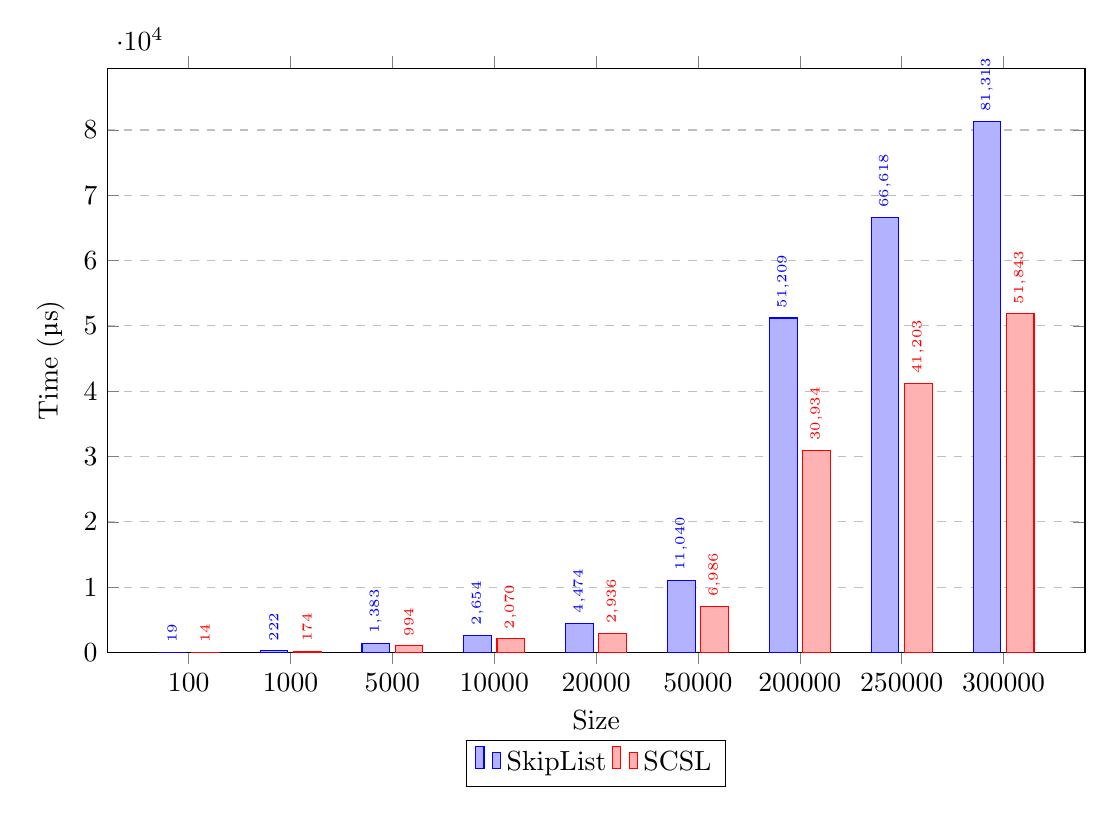
\begin{tikzpicture}
\begin{axis}[
    ybar,
    bar width=10pt,
    width=14cm,
    height=9cm,
    enlarge x limits=0.1,
    xlabel={Size},
    ylabel={Time (µs)},
    symbolic x coords={100,1000,5000,10000,20000,50000,200000,250000,300000},
    xtick=data,
    legend style={at={(0.5,-0.15)},anchor=north,legend columns=2},
    nodes near coords,
    every node near coord/.append style={font=\tiny, rotate=90, anchor=west},
    ymin=0,
    ymajorgrids=true,
    grid style=dashed
]
\addplot+[style={blue,fill=blue!30}] coordinates {
    (100,19) (1000,222) (5000,1383) (10000,2654)  (20000,4474) (50000,11040) (200000,51209) (250000,66618) (300000,81313)
};
\addplot+[style={red,fill=red!30}] coordinates {
    (100,14) (1000,174) (5000,994) (10000,2070)  (20000,2936) (50000,6986) (200000,30934) (250000,41203) (300000,51843)
};

\legend{SkipList, SCSL}
\end{axis}
\end{tikzpicture}
\caption{Insertion Time Comparison Between SkipList and SCSL at Different Scales(smaller is better) in Macos}
\end{figure}

\begin{figure}[htbp]
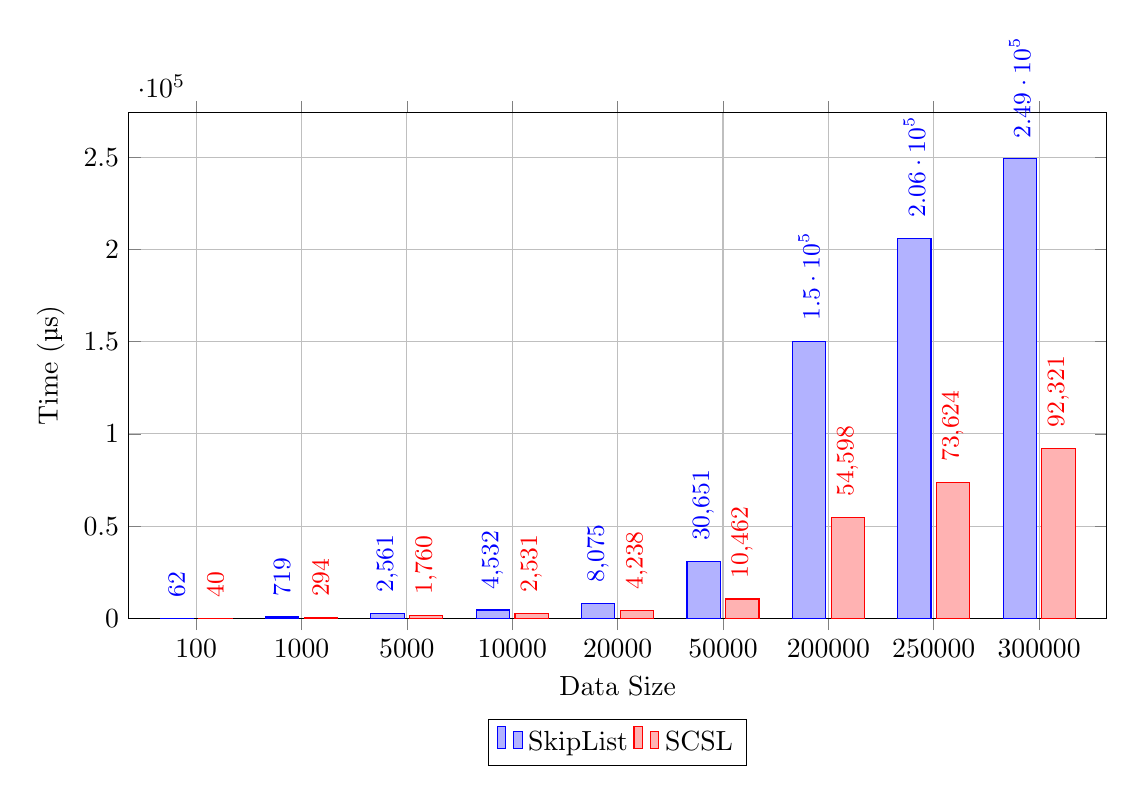
\begin{tikzpicture}
\begin{axis}[
    width=14cm,
    height=8cm,
    ybar,
    bar width=12pt,
    symbolic x coords={100,1000,5000,10000,20000,50000,200000,250000,300000},
    xtick=data,
    xlabel={Data Size},
    ylabel={Time (µs)},
    legend style={at={(0.5,-0.2)},anchor=north,legend columns=-1},
    enlarge x limits=0.08,
    ymin=0,
    grid=major,
    nodes near coords,
    nodes near coords style={font=\small, anchor=west, rotate=90, xshift=4pt},
]

\addplot coordinates {(100,62) (1000,719) (5000,2561) (10000,4532) (20000,8075) (50000,30651) (200000,150126) (250000,206036) (300000,249135)};
\addplot coordinates {(100,40) (1000,294) (5000,1760) (10000,2531) (20000,4238) (50000,10462) (200000,54598) (250000,73624) (300000,92321)};

\legend{SkipList, SCSL}
\end{axis}
\end{tikzpicture}
\caption{Insertion Time Comparison Between SkipList and SCSL at Different Scales(smaller is better) in Server}
\end{figure}

We evaluated the standard skip list and SCSL with a maximum level of 16. Figure 3 presents the insertion performance comparison between the standard skip list and simple cache skip list in a Macbook. It shows that under small scale of data (< 1000) simple cache skip list can speed up to 1.28~1.39 times, and under medium scale (over 20000) , it can speed up to 1.55~1.65 times, as the scale increasing, the more benefit for performance. Figure 4 also shows that, in server computer, the simple cache skip list can speed up even 3 times.
\begin{table}
\begin{tabular}{lrrr}
\toprule
Test Case & Cache References & Cache Misses & Cache Miss Rate \\
\midrule
SCSL & 51,567,218 & 459,636 & 0.89\% \\
Standard Skip List & 142,249,678 & 47,251,323 & 33.22\% \\
\bottomrule
\end{tabular}
\caption{Cache Performance Comparison Between SCSL and standard Skip list in server computer}
\end{table}

As shown in the table above(table 1), the standard skip list in the test achieves a 33.22\% cache-miss rate, whereas SCSL has only a 0.89\% cache-miss rate. It also proves that adding arrays to data nodes can work very well.



\section{Conclusions}
We present a new method to implement a cache-sensitive skip list, SCSL, which only changes a single element in the data-level nodes to an array. SCSL effectively leverages CPU caches by using data stored in continuous memory, and the algorithm is simple. Additionally, the performance results are also significant.
\begin{thebibliography}{9} 
\bibitem{ref1}
      Skip Lists: A Probabilistic Alternative to Balanced Trees
\bibitem{ref2}
      Google. LevelDB. Available online: https://github.com/google/leveldb (accessed on 20 July 2023).
\bibitem{ref3}
      Facebook. RocksDB. Available online: http://rocksdb.org/ (accessed on 20 July 2023).
\bibitem{ref4}
      Apache. Welcome to Apache HBase™. Available online: https://hbase.apache.org/ (accessed on 20 July 2023).
\bibitem{ref5}
      Cache-Sensitive Skip List: Efficient Range Queries on modern CPUs - informatik.hu-berlin.de.
\bibitem{ref6}
      ESL: A High-Performance Skiplist with Express Lane  https://www.mdpi.com/2076-3417/13/17/9925
\bibitem{ref7}
	Redis, Accessed: 2024-01-09.
\end{thebibliography}
\end{document}